\chapter{Introduction}\label{introduction}

This document is intended for developers who are creating user interfaces for EnergyPlus.~ It provides an overview of the essentials of the input-output structure of EnergyPlus and describes the parts of each in detail.

\begin{figure}[hbtp] % fig 1
\centering
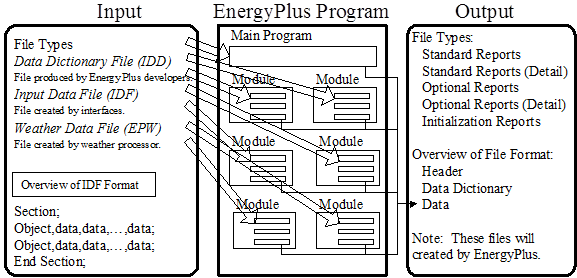
\includegraphics[width=0.9\textwidth, height=0.9\textheight, keepaspectratio=true]{media/image001.png}
\caption{EnergyPlus Input/Output Overview \protect \label{fig:energyplus-inputoutput-overview}}
\end{figure}

The diagram shown above should give the reader an overall picture of input-output in EnergyPlus.~ It can be seen as a linear process that includes the following steps:

1)~~~The user enters building description (including internal space gains, HVAC arrangements, and Plant equipment properties) using the interface of their choice.~ In addition, the user specifies which non-default reports are desired and any optional variables from a predefined list of available simulation quantities.

2)~~~The interface program writes the Input Data File (IDF) file, which includes the specification of any report items desired by the user.

3)~~~EnergyPlus processes both the Input Data Dictionary (IDD) and the Input Data File (IDF) files with the ``InputProcessor''.~ The InputProcessor uses the specifications/rules defined in the IDD and interprets the IDF raw data.~ The InputProcessor is really quite ``dumb'' and only understands a few things about each field (alpha or numeric) qualified by certain key elements in the IDD (\textbackslash{} comments which are discussed later).

4)~~~Each module in EnergyPlus has one or several routines (normally called ``GetInput'' routines) that obtain the information from the IDF file data.~ These subroutines decode the portion of the IDF file that is pertinent to the local module.~ These GetInput routines are more context sensitive than the InputProcessor and may perform further error detection.~ For example, the cooling coil module may read in the coil type and its associated parameters (number of rows, tube diameter, fin spacing, etc.).

5)~~~EnergyPlus performs the simulation elements specified in the IDF.~ Output is generated as a continuous stream (for the most part) and must be interpreted into a more cohesive form by output processing.~ The user has control over which outputs are produced and when/how often.

6)~~~EnergyPlus produces output as required by the user into one of the output files.~ These files can be readily processed into spreadsheet formats for graphing and other summarizing.
